\subsection{球冠}\label{subsec:2-6}

\subsubsection{球冠}

观察天象的天文台的屋顶(图 \ref{fig:ltjh-2-51}),光学透镜和反射镜的凹、凸面,都是球面的一部分。

\begin{figure}[htbp]
    \centering
    \begin{minipage}[b]{7cm}
        \centering
        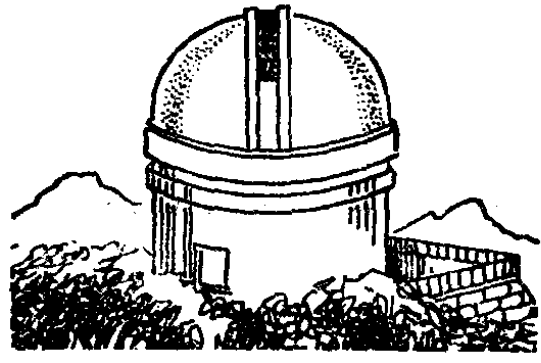
\includegraphics[width=5cm]{../pic/ltjh-ch2-51.png}
        \caption{}\label{fig:ltjh-2-51}
    \end{minipage}
    \qquad
    \begin{minipage}[b]{7cm}
        \centering
        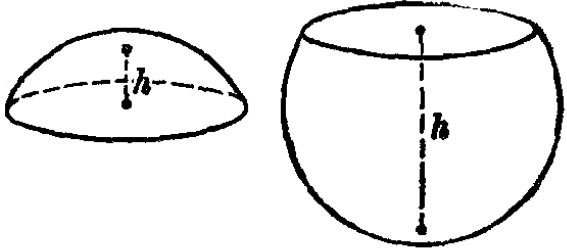
\includegraphics[width=5cm]{../pic/ltjh-ch2-52.png}
        \caption{}\label{fig:ltjh-2-52}
    \end{minipage}
\end{figure}

球面被平面所截得的一部分叫做\zhongdian{球冠},截得的圆叫做\zhongdian{球冠的底}。
垂直于截面的直径被截得的一段叫做\zhongdian{球冠的高}(图 \ref{fig:ltjh-2-52})。

球冠也可以看作一段圆弧绕经过它的一个端点的直径旋转所成的曲面。

我们完全可以仿照求半球面面积的方法,求出球冠的面积。
将图 \ref{fig:ltjh-2-49} 看作是由半径为 $R$ 的球截得的球冠,那么 $ON$ 就是球冠的高,
用 $h$ 表示,这样就得到下面的定理:

\begin{dingli}[定理][dl:qgdmj]
    球冠的面积等于截成它的球面上大圆周长与球冠的高的积。
    \begin{center}
        \framebox[10em]{$\bm{S_\text{球冠} = 2\pi Rh}$。}
     \end{center}
    \vspace*{-2.5em}即
\end{dingli}\vspace{1em}

这个公式,对于小于半球面的球冠,半球面,大于半球面的球冠及整个球面都是适用的。
当 $h = 2R$ 时,就是球面的面积 $4\pi R^2$。


\liti 运油车的油罐是由一个圆筒与两个相同的球冠形部分组成的。 油罐的尺寸如图 \ref{fig:ltjh-2-53}(单位:m)。
求制造这样一个油罐需要多少平方米钢板(精确到 $0.1\;\pfm$)。

\begin{wrapfigure}[8]{r}{6.5cm}
    \centering
    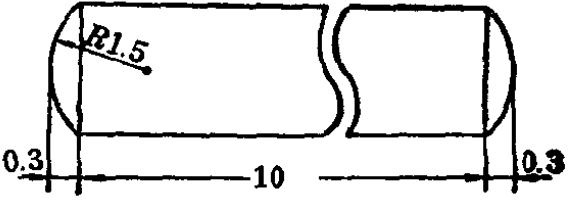
\includegraphics[width=6cm]{../pic/ltjh-ch2-53.png}
    \caption{}\label{fig:ltjh-2-53}
\end{wrapfigure}

\jie 设圆筒半径为 $r$,它也是球冠的底的半径。由平面几何知识可得

\qquad $r^2 = 0.3 (2 \times 1.5 - 0.3)$,

$\therefore$ \quad $r = 0.9$ (m)。

油罐圆筒部分面积:

\qquad $S_1 = 2\pi rh_1 = 2\pi \times 0.9 \times 10 \approx 56.52\;(\pfm)$;

两个球冠部分的面积:

\qquad $2S_2 = 2 \times 2\pi Rh_2 = 2 \times 2\pi \times 1.5 \times 0.3 \approx 5.65 \; (\pfm)$。

油罐的总面积:

\qquad $S = S_1 + 2S_2 = 56.52 + 5.65 \approx 62.2 \; (\pfm)$。

答:制造这样一个油罐要用钢板约 62.2 平方米。


\liti 我国土地面积约为 $9.60 \times 10^6 \; \pfqm$,大部分位于地球北温带。 求我国领土是北温带面积的百分之几。

\jie 图 \ref{fig:ltjh-2-54} 表示经过地球南、北极的一个截面。 $N$ 是北极,点 $G$ 在赤道上,点 $A$、$B$ 在北回归线上,
$C$、$D$ 在北极圈上。 $CD \pingxing AB$, $ON \perp AB$, $ON \perp CD$。

北温带的面积

$\begin{aligned}
    S_\text{北温带} &= S_{\text{球冠} ABN} - S_{\text{球冠} CDN} \\
        &= 2\pi R \cdot EN - 2\pi R \cdot FN \\
        &= 2\pi R (EN - FN) \\
        &= 2\pi R (OF - OE) \juhao
\end{aligned}$

$\because$ \quad $\begin{aligned}[t]
    OF - OE &= OC \sin OCF - OA \sin OAE \\
        &= 6.37 \times 10^3 (\sin 66.5^\circ - \sin 23.5^\circ) \\
        &= 6.37 \times 10^3 (0.9171 - 0.3987) \\
        &\approx 3.302 \times 10^3 \; (\qianmi) \douhao
\end{aligned}$

$\therefore$ \quad $S_\text{北温带} = 2 \times 3.142 \times 6.37 \times 10^3 \times 3.302 \times 10^3 \approx 1.32 \times 10^8 \; (\qianmi)$。

\begin{enhancedline}
\hspace{4em} $\dfrac{9.60 \times 10^6 \times 100}{1.32 \times 10^8 \times 100} \approx 7.27 \%$。

答:我国领土约是北温带面积的百分之七点二七。
\end{enhancedline}

\begin{figure}[htbp]
    \centering
    \begin{minipage}[b]{7cm}
        \centering
        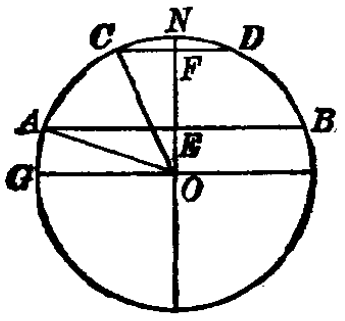
\includegraphics[width=4.5cm]{../pic/ltjh-ch2-54.png}
        \caption{}\label{fig:ltjh-2-54}
    \end{minipage}
    \qquad
    \begin{minipage}[b]{7cm}
        \centering
        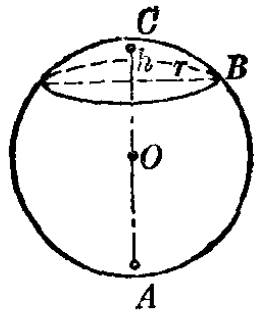
\includegraphics[width=4cm]{../pic/ltjh-ch2-subsec6-lx1-01.png}
        \caption*{(第 1 题)}
    \end{minipage}
\end{figure}

\begin{lianxi}

\xiaoti{求证: $S_\text{球冠} =  \pi (r^2 + h^2)$, 其中 $r$ 是球冠的底的半径,$h$ 是球冠的高。}

\xiaoti{有一条半径为 $R$ 的弧,度数是 $120^\circ$,它绕经过弧的中点的直径旋转得到一个球冠。求这个球冠的面积。}

\end{lianxi}



\subsubsection{旋转面和旋转体}

\begin{wrapfigure}[10]{r}{4.5cm}
    \centering
    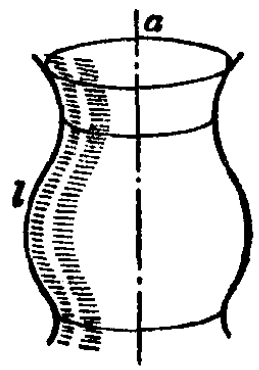
\includegraphics[width=3.5cm]{../pic/ltjh-ch2-55.png}
    \caption{}\label{fig:ltjh-2-55}
\end{wrapfigure}

前面我们学过的圆柱、圆锥、圆台的侧面,球面及球冠等,都是平面内的一条曲线绕一条定直线旋转而成的。

一条平面曲线(包括直线)绕它所在的平面内的一条定直线旋转所形成的曲面叫做\zhongdian{旋转面}。
这条定直线叫做\zhongdian{旋转轴}。无论旋转到什么位置,这条曲线都叫做旋转面的\zhongdian{母线}。
图 \ref{fig:ltjh-2-55} 中,直线 $a$ 是旋转轴,曲线 $l$ (不论旋转到什么位置)是母线。

如果母线是与旋转轴平行的直线,那么形成的旋转面叫做\zhongdian{圆柱面}(图 \ref{fig:ltjh-2-56} 甲)。
如果母线是和旋转轴斜交的直线,那么形成的旋转面叫做\zhongdian{圆锥面}(图 \ref{fig:ltjh-2-56} 乙),
这时,母线和轴的交点叫做\zhongdian{圆锥面的顶点}。
以前学过的圆柱、圆锥、圆台的侧面可分别看成是圆柱面、圆锥面被垂直于轴的平面截得的一部分。

如果一个圆,绕同一平面内与它不相交的一条直线旋转,那么形成的旋转面叫做\zhongdian{环面}(图 \ref{fig:ltjh-2-56} 丙)。

\begin{figure}[htbp]
    \centering
    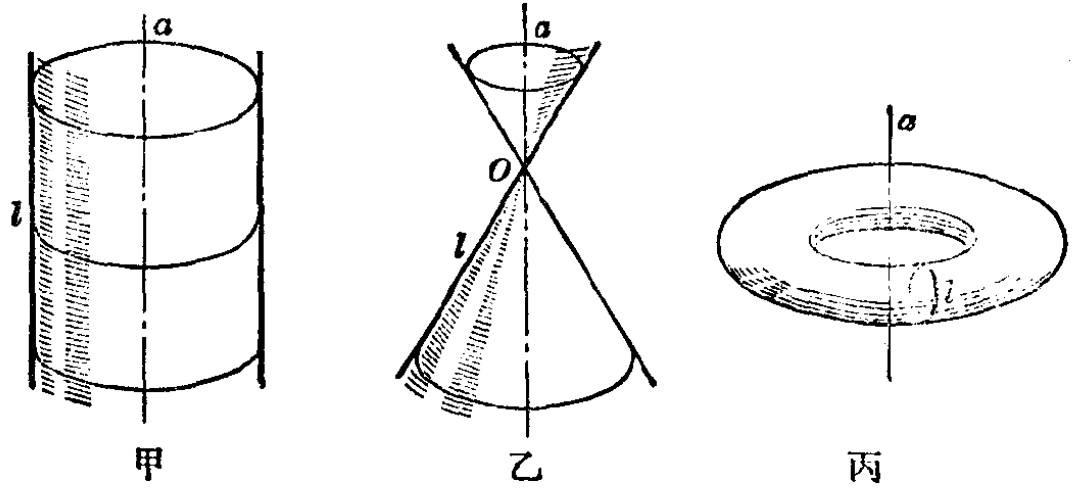
\includegraphics[width=12cm]{../pic/ltjh-ch2-56.png}
    \caption{}\label{fig:ltjh-2-56}
\end{figure}

封闭的旋转面围成的几何体,叫做\zhongdian{旋转体}。 这时,旋转面的轴也叫\zhongdian{旋转体的轴}。
圆柱、圆锥、圆合、球都是旋转体。 环面所围成的几何体也是旋转体,它叫做\zhongdian{环体},简称\zhongdian{环}。
例如充气的车轮内胎就呈环体形。


\begin{lianxi}

\xiaoti{举出一些旋转面和旋转体的实例。}

\xiaoti{圆柱和圆柱面、圆锥和圆锥面有何区别?}

\end{lianxi}

